\documentclass[review,11pt,a4paper]{elsarticle}
\usepackage[margin=2.4cm]{geometry}
\usepackage{booktabs}
\usepackage{caption}
\usepackage[hidelinks]{hyperref}

\captionsetup{font=small,labelfont=bf,skip=4pt}
\graphicspath{{../figures/}}
\setlength{\parskip}{3pt}

\journal{Computational Materials Science}

\begin{document}

\begin{frontmatter}

\title{An Artificial-Intelligence-Based Materials Informatics Framework for the Accelerated Discovery of Calcium Phosphate Biomaterials as Candidate Scaffolds for Bone Tissue Engineering}

\author[unair]{Soegianto Soelistiono\corref{cor1}}
\ead{soegianto@fst.unair.ac.id}
\author[unair]{Herri Trilaksana}
\author[unair]{Yhosep Gita Yhun Yhuwana}
\author[aru]{Bernardi Pranggono}

\affiliation[unair]{organization={Department of Physics, Faculty of Science and Technology, Universitas Airlangga}, city={Surabaya}, postcode={60115}, country={Indonesia}}
\affiliation[aru]{organization={School of Computing and Information Science, Anglia Ruskin University}, city={Cambridge}, country={United Kingdom}}
\cortext[cor1]{Corresponding author}


\begin{abstract}
Bone defects arising from trauma, degenerative disease, and congenital abnormalities remain a major clinical challenge. Calcium phosphate biomaterials are attractive scaffold candidates owing to their biocompatibility, bioactivity, and osteoconductivity, yet conventional trial-and-error discovery is time- and cost-intensive. Here we present an end-to-end Materials Informatics framework that integrates five open materials databases (Materials Project, AFLOW, Crystallography Open Database, PubChem, OQMD) with artificial intelligence to accelerate the discovery of calcium phosphate biomaterials for bone tissue engineering scaffolds. A curated dataset of 2{,}885 entries spanning 950 unique compositions was assembled and audited. Physicochemical descriptors (Ca/P ratio, average electronegativity, valence electron concentration, molecular weight, cell volume, density) were engineered and multicollinearity was controlled ($|r| > 0.85$, VIF $> 10$). Predictive models were evaluated under a leakage-resistant protocol: composition-grouped cross-validation on reduced chemical formulas (so that polymorphs and formula multiples never straddle folds), nested hyperparameter selection, and composition-only descriptors in discovery settings (no cell volume or density, which are unavailable for unknown materials). The formation-energy model (nested SVR) attains $R^2 = 0.48$ (MAE 0.27 eV/atom) across all computed entries and $R^2 = 0.58$ within the phosphate family; applied to an external database at matching compositions, it attains $R^2 = 0.88$. The models reproduce experimental standard formation enthalpies and densities of six calcium phosphate phases with MAEs of 0.25 eV/atom and 0.18 g/cm$^3$, respectively. Absolute accuracy is modest compared with graph-neural-network state of the art (MAE $\approx$ 0.03--0.1 eV/atom), a gap we discuss explicitly. Multi-objective ranking (TOPSIS and VIKOR under three weighting scenarios, with Shannon-entropy sensitivity analysis) places fluorapatite, carbonated apatite, $\beta$-TCP, and hydroxyapatite among the leading candidates; the ranking criteria are deliberately derived from bone-tissue design requirements, and the analysis states explicitly that no resorption criterion is represented---so $\beta$-TCP's clinical resorbability, though not rewarded, does not prevent its top placement on thermodynamic and compositional grounds. Independent experimental validation of the models is provided: the formation-energy model reproduces experimental standard formation enthalpies of six calcium phosphate phases with MAE 0.25 eV/atom, and the density model reproduces experimental densities with MAE 0.18 g/cm$^3$; at matching compositions, the formation-energy model transfers across databases with $R^2 = 0.88$ (280 OQMD entries). SHAP analysis identifies the oxygen fraction and molecular weight as the dominant descriptors, with the caveat that part of their importance separates the phosphide and phosphate families. The framework is fully replicable (versioned dataset with checksums, open tooling) and provides a foundation for an AI-assisted biomaterial discovery platform.

\end{abstract}

\begin{keyword}
materials informatics \sep machine learning \sep calcium phosphate \sep bone tissue engineering \sep scaffold \sep multi-criteria decision making \sep SHAP
\end{keyword}
\end{frontmatter}

%=============================================================
\section{Introduction}

Bone defects caused by trauma, degenerative diseases, infection, congenital abnormalities, and aging remain a major burden on healthcare systems, often leading to loss of mechanical function and reduced quality of life~\cite{farag2023}. Bone tissue engineering, which combines biomaterials, cells, and biological factors, has emerged as a promising strategy in which the biomaterial acts as a scaffold that provides structural support and a suitable microenvironment for cell adhesion, proliferation, and differentiation~\cite{farag2023}. Calcium phosphate ceramics remain the materials of choice because their mineral composition resembles natural bone, and they are biocompatible, bioactive, and osteoconductive~\cite{vaiani2023}.

Advances in scaffold fabrication, particularly 3D printing, enable scaffolds with tailored geometry, porosity, and internal architecture~\cite{premananth2024}. Machine learning has been integrated into the optimization of composite scaffolds such as PLA/cHAP, improving mechanical properties and fabrication parameters~\cite{omigbodun2024}. Additive manufacturing research increasingly combines biodegradable polymers and ceramics for patient-specific structures~\cite{zhu2025}, supported by multiscale biomechanics-driven design pipelines~\cite{hou2026} and modeling/simulation approaches that make scaffold development more systematic than conventional trial-and-error~\cite{vasudev2026}.

In parallel, artificial intelligence (AI) has begun to accelerate biomaterial design through materials data analysis, process optimization, property prediction, and automated candidate recommendation~\cite{martelli2025,logeshwaran2024,gokcekuyu2024}. Data-driven approaches have been used to predict material properties, biomolecular stability, and product characteristics using materials databases and machine learning algorithms~\cite{kang2023,kalejaye2024,hayashi2023}, and AI has transformed pharmaceutical formulation and manufacturing workflows in an analogous manner~\cite{nizamuddin2025,han2025,vora2023,gholap2024}.

Nevertheless, most reported work focuses on isolated stages---biomaterial development, manufacturing optimization, or the application of AI to a specific step---whereas a comprehensive Materials Informatics framework that integrates data acquisition, descriptor engineering, AI analysis, multi-objective evaluation, and interpretable recommendation remains rare. As a preliminary step, our group developed a data-driven discovery workflow for calcium phosphate scaffolds using materials informatics and machine learning clustering, screening hundreds of compounds based on thermodynamic stability, crystal structure, density, and electronic properties~\cite{soelistiono2026}. That study demonstrated that multi-objective descriptor balancing yields more representative material rankings than single dominant parameters, but it did not yet constitute a systematic, replicable framework.

In this work, we address this gap by developing and validating an end-to-end Materials Informatics framework with the following contributions: (i) an audited multi-source dataset of 2{,}885 calcium phosphate entries spanning 950 unique compositions; (ii) descriptor engineering with explicit multicollinearity control; (iii) predictive models for formation energy and density, evaluated under a leakage-resistant protocol (reduced-formula grouping, nested cross-validation, composition-only descriptors); (iv) multi-objective ranking with TOPSIS/VIKOR and Shannon-entropy sensitivity analysis; and (v) independent validation of the models against experimental thermochemistry and crystallographic densities.

%=============================================================
\section{Methods}

\subsection{Data acquisition}
Five open data sources were queried (Table~\ref{tab:sumber}): the Materials Project REST API (CC-BY 4.0), AFLOW (AFLUX REST API), the Crystallography Open Database (COD, CC0, queried over HTTP), PubChem (PUG REST, public domain), and OQMD (oqmdapi, flaky server handled with long retries and per-composition caching). Chemical systems queried were Ca--P, Ca--P--O, Ca--P--O--H, Ca--P--O--C (carbonated apatite), and Ca--P--O--F (fluorapatite). Access dates, versions, and licenses were recorded for every source (Supplementary).

\begin{table}[ht]
\centering\small
\caption{Data sources, licenses, and entries retained in the consolidated dataset.}
\label{tab:sumber}
\begin{tabular}{llcl}
\toprule
Source & Access & License & Entries \\
\midrule
Materials Project & API (key) & CC-BY 4.0 & 57 \\
AFLOW (AFLUX) & REST, no key & cite Curtarolo et al. & 234 \\
COD (crystallography.net) & HTTP, no key & CC0 & 2{,}304 \\
PubChem & PUG REST, no key & public domain & 13 \\
OQMD & oqmdapi, no key & cite Kirklin et al. & 280 \\
\midrule
\textbf{Total} & & & \textbf{2{,}885} \\
\bottomrule
\end{tabular}
\end{table}

\subsection{Preprocessing and descriptor engineering}
Non-physical values (negative density, non-positive cell volume) were nulled (4 rows). Outliers were detected with IQR$\times$3 and $|z|>4$ rules and \emph{retained} when physically plausible, with per-case decisions recorded. Units were standardized to SI (GPa, g/cm$^3$, eV/atom, \AA$^3$). Theoretical density for COD entries was computed as $\rho = MZ/(N_A V_\mathrm{cell})$. Descriptors included the Ca/P atomic ratio, average electronegativity (EN$_\mathrm{avg}$) and electronegativity range (EN$_\mathrm{diff}$), valence electron concentration (VEC), molecular weight, cell volume, and density. Redundant descriptors were removed ($|r| > 0.85$ with EN$_\mathrm{avg}$, VIF $> 10$): EN$_\mathrm{diff}$ ($r=0.889$) and VEC ($r=0.902$).

\subsection{Machine learning}
The modeling subset comprised entries from computational sources (Materials Project, AFLOW, OQMD). Regression targets were formation energy (eV/atom) and density (g/cm$^3$); models included random forest (RF), XGBoost, gradient boosting, and support vector regression (SVR). Three methodological safeguards against data leakage were applied. \emph{(i) Grouping by reduced formula:} cross-validation groups were defined by the greatest-common-divisor-reduced composition (e.g., Ca$_5$P$_3$O$_{12}$F and Ca$_{10}$F$_2$O$_{24}$P$_6$ share one group), so that polymorphs and integer multiples of a formula never straddle folds. \emph{(ii) Nested cross-validation:} SVR hyperparameters ($C \in \{1,10,50\}$, $\gamma \in \{0.01,0.05,0.1\}$, $\varepsilon \in \{0.05,0.1\}$) were selected in an inner 5-fold grouped CV within each outer fold; reported scores are the outer-loop estimates. \emph{(iii) Discovery-appropriate features:} the headline model uses composition-only descriptors (Ca/P, average electronegativity, molecular weight, element fractions); cell volume and density---which are unavailable for unknown materials, and which make the density ``model'' a near-tautology $\rho = MZ/(N_A V)$---are used only in a clearly labeled screening scenario for ranking existing database entries. Because formation-energy scales differ systematically between databases (AFLOW deviates from Materials Project/OQMD by up to 0.8 eV/atom for phosphides, whereas the latter two agree within 0.02 eV/atom on overlapping compositions), the external test uses OQMD entries, whose compositions, however, all appear in the training sources; the test is therefore a same-composition cross-database transfer test, not a composition-extrapolation test, and is reported as such. A scaffold-suitability label (E$_f \leq -2.5$ eV/atom, Ca/P $\in [1.0, 2.1]$, density $\in [0.5, 4.5]$ g/cm$^3$) is computed for completeness but is a semi-deterministic function of its own input features and is neither reported as a predictive achievement nor used as a ranking criterion.

\subsection{Multi-criteria decision making (MCDM)}
Five criteria were defined: (C1) thermodynamic stability (formation energy, lower is better); (C2) density within the clinically processable band $[1.0, 3.2]$ g/cm$^3$ (zero penalty inside; a scaffold reaches bone-like stiffness through porosity---Gibson--Ashby---not by matching bone density); (C3) Ca/P proximity to 1.67 (bone mineral); (C4) Young's modulus proximity to 15 GPa (mid-range of cortical bone), derived as $E = 9KG/(3K+G)$ where bulk and shear moduli were available and median-imputed otherwise (recorded decision); and (C5) band gap (capped at 5 eV, metallic entries penalized, measured values only). A classifier-derived suitability score was deliberately \emph{excluded} because it is a semi-deterministic function of the same inputs as C1--C3 (double counting). Candidates were ranked with TOPSIS and VIKOR ($v=0.5$) under three weighting scenarios (balanced; stability-dominant; mechanics-dominant). Sensitivity was tested with Shannon-entropy weighting computed on the three imputation-free criteria, keeping manual weights for the imputed criteria; rank consistency was quantified with Spearman correlation.

\subsection{Interpretability and validation}
SHAP (TreeExplainer) values and permutation importance were computed for the E$_f$ and density models. Reference phases (hydroxyapatite, fluorapatite, $\beta$-TCP, $\alpha$-TCP, tetracalcium phosphate, carbonated apatite) were compared against experimental literature values for density, lattice parameters, and standard formation enthalpies. Structures of the top-5 candidates were exported (POSCAR, CIF) and Quantum ESPRESSO input files (scf/relax, PSL 1.0.0 pseudopotentials) were prepared for subsequent DFT validation.

%=============================================================
\section{Results}

\subsection{Dataset and design space}
The consolidated dataset contains 2{,}885 entries and 950 unique compositions (target $\geq 500$ met). Completeness: cell volume and space group are available for 99.5\% of entries; formation energies for 19.8\% (computational sources only); elastic moduli for 0.3\% ($n=9$). Reference phases are well represented (54 hydroxyapatite entries, 17 TCP entries). Correlation analysis identified two redundant descriptor pairs with EN$_\mathrm{avg}$ ($r > 0.85$), confirmed by VIF values up to 24. Principal component analysis (Fig.~\ref{fig:pca}) captures 61.1\% of the variance in the first two components, and the chemical families (apatites, TCP, DCP, OCP, metaphosphates) form recognizable regions of the design space. Clustering is robust: K-means ($k=5$, silhouette 0.552) is highly consistent with hierarchical Ward clustering (ARI = 0.907), and HDBSCAN identifies 17 dense clusters with 1{,}266 noise points (Supplementary). The average density per family ranges from 1.5 g/cm$^3$ (monocalcium phosphates) to 3.1 g/cm$^3$ (hydroxyapatite family; Fig.~\ref{fig:densitas}), consistent with crystallographic expectations.

A source-bias check (Fig.~\ref{fig:tsne}) shows that 94\% of the five nearest neighbors of an entry come from the same database, indicating that clusters are partly source-driven (experimental COD data vs.\ computed MP/AFLOW data). This motivated restricting modeling to the computational subset and the use of composition-grouped splits.

\begin{figure}[ht]
\centering
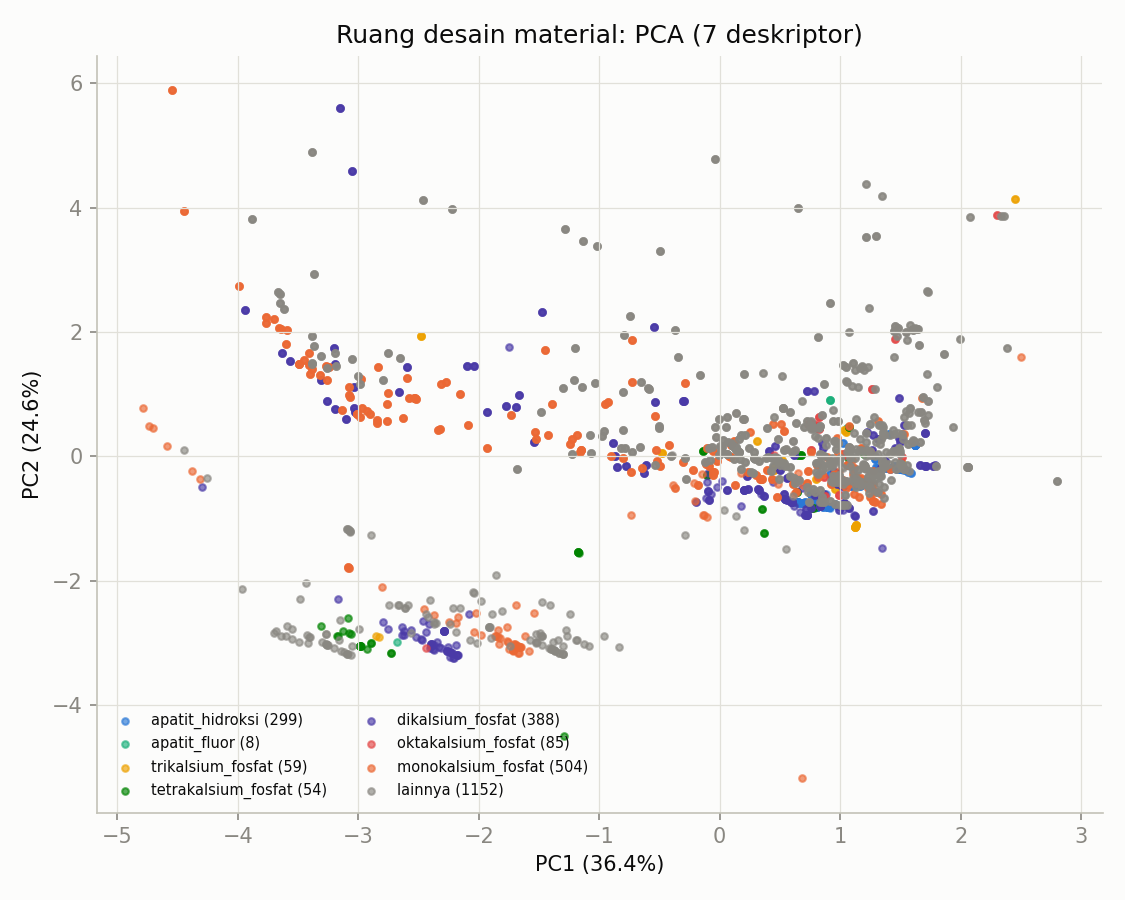
\includegraphics[width=0.62\textwidth]{fig_pca_kelompok.png}
\caption{Design space of calcium phosphates mapped by PCA over seven physicochemical descriptors, colored by material family.}
\label{fig:pca}
\end{figure}

\begin{figure}[ht]
\centering
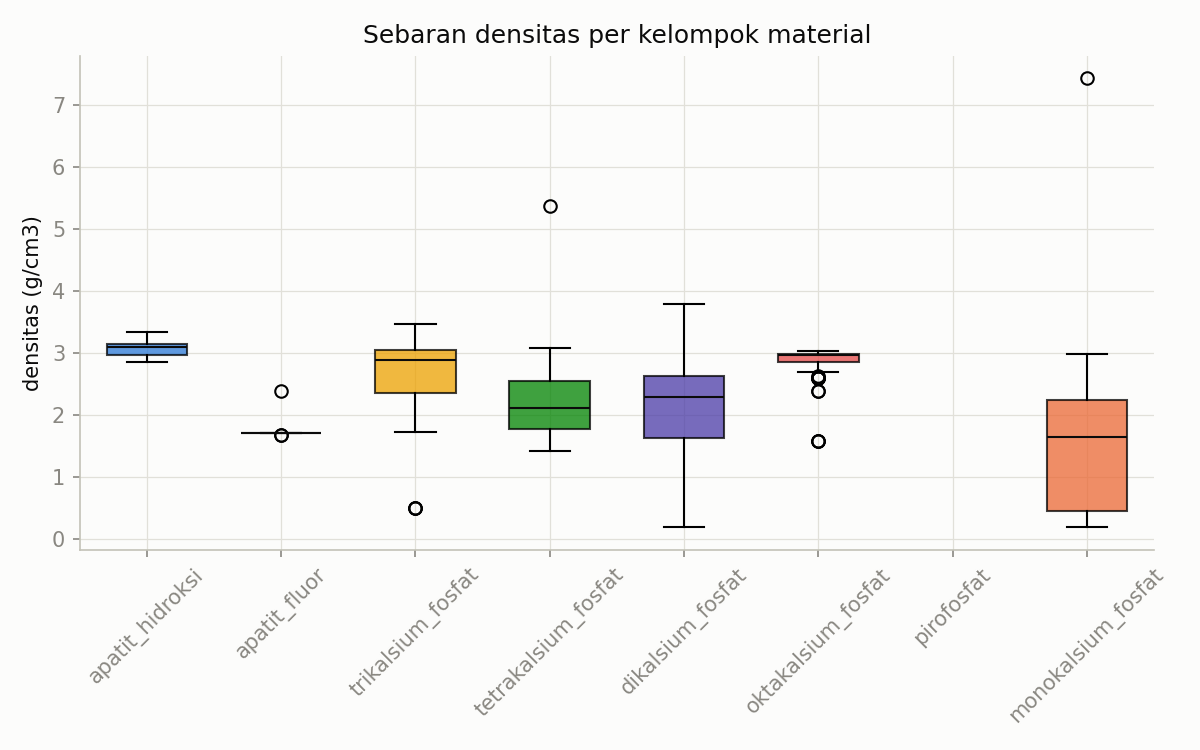
\includegraphics[width=0.62\textwidth]{fig_densitas_kelompok.png}
\caption{Density distribution per material family. Hydroxyapatite-family phases concentrate near 3.0--3.2 g/cm$^3$, close to bone mineral.}
\label{fig:densitas}
\end{figure}

\begin{figure}[ht]
\centering
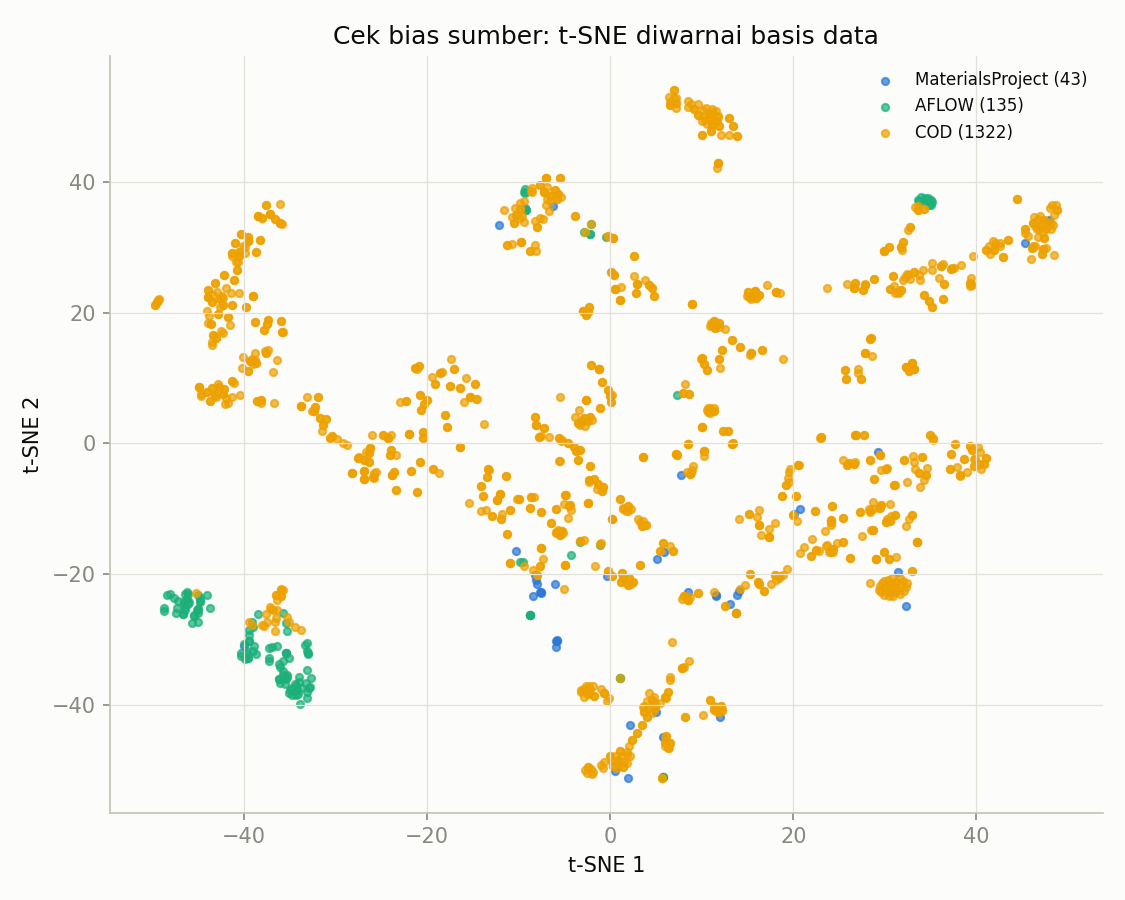
\includegraphics[width=0.62\textwidth]{fig_tsne_sumber.png}
\caption{t-SNE embedding colored by data source, revealing source-driven separation (94\% same-source nearest neighbors) that motivates the computational-only modeling subset.}
\label{fig:tsne}
\end{figure}

\subsection{Predictive models}
Table~\ref{tab:ml} reports all metrics under the leakage-resistant protocol (reduced-formula grouping; nested CV for SVR). With composition-only descriptors---the honest discovery setting---the nested SVR attains $R^2 = 0.483$ (MAE 0.265 eV/atom) across all 571 computed entries, and $R^2 = 0.580$ (MAE 0.176 eV/atom) within the phosphate family alone, confirming that part of the headline $R^2$ previously obtainable with structure-informed features reflected the trivial separation of phosphides from phosphates. A structure-informed variant (volume + density as features, valid only for screening existing database entries, $n=291$) attains $R^2 = 0.489$. The composition-only density model attains only $R^2 = 0.174$---expected, since crystal density is governed by packing, not stoichiometry; the $[M, V]$-based variant is a near-tautology ($\rho = MZ/N_A V$, with $Z$ unobserved) and is reported as a data-consistency check, not a model. On the external OQMD database at matching compositions, the composition-only formation-energy model attains $R^2 = 0.883$ (MAE 0.254 eV/atom); we emphasize that all OQMD compositions also occur in the training sources, so this is a same-composition cross-database transfer test, not composition extrapolation. The suitability label, being a semi-deterministic function of its own features, is not reported as a predictive result. Band gap could not be predicted from composition descriptors ($R^2 < 0$); imputation was therefore abandoned (recorded decision).

\begin{table}[ht]
\centering\small
\caption{Metrics under the leakage-resistant protocol: reduced-formula grouping, nested CV for SVR, composition-only features unless stated otherwise.}
\label{tab:ml}
\begin{tabular}{llccc}
\toprule
Task & Model & $R^2$ & RMSE & MAE \\
\midrule
Formation energy, all entries ($n=571$) & SVR (nested) & 0.483 & 0.465 & 0.265 \\
Formation energy, phosphates only ($n=215$) & SVR & 0.580 & 0.284 & 0.176 \\
Formation energy, screening variant ($n=291$) & SVR (nested) & 0.489 & 0.448 & 0.242 \\
Cross-database, same compositions ($n=280$) & SVR & 0.883 & 0.385 & 0.254 \\
Density, composition-only ($n=571$) & Random forest & 0.174 & 0.400 & 0.264 \\
\bottomrule
\end{tabular}
\end{table}

\subsection{Multi-objective ranking}
TOPSIS and VIKOR were combined across three weighting scenarios (six rankings in total) to produce a robust average rank. Shannon-entropy weighting (computed on the three imputation-free criteria) yields a Spearman correlation of 0.974 with the manual weighting, confirming the robustness of the ranking. The top candidates after polymorph deduplication are listed in Table~\ref{tab:top}: fluorapatite leads, followed by carbonated apatite, $\beta$-TCP, and hydroxyapatite, with tetracalcium phosphate, monetite, and octacalcium phosphate completing the clinically relevant shortlist.

\begin{table}[ht]
\centering\small
\caption{Top 15 candidate biomaterials (polymorphs deduplicated; average rank of TOPSIS and VIKOR across three weighting scenarios; lower rank is better).}
\label{tab:top}
\begin{tabular}{lllcccc}
\toprule
Formula & Source & Family & Rank & E$_f$ (eV/at) & $\rho$ (g/cm$^3$) & Ca/P \\
\midrule
Ca$_5$P$_3$O$_{12}$F & MP & fluorapatite & 1.3 & $-3.42$ & 3.10 & 1.67 \\
Ca$_{10}$P$_6$CO$_{27}$ & MP & carbonated apatite & 4.3 & $-3.25$ & 3.05 & 1.67 \\
Ca$_3$(PO$_4$)$_2$ & MP & $\beta$-TCP & 4.8 & $-3.32$ & 2.98 & 1.50 \\
Ca$_5$P$_3$HO$_{13}$ & MP & hydroxyapatite & 5.5 & $-3.22$ & 3.18 & 1.67 \\
Ca$_{10}$F$_2$O$_{24}$P$_6$ & AFLOW & fluorapatite & 9.7 & $-3.03$ & 3.10 & 1.67 \\
Ca$_4$P$_2$O$_9$ & MP & TTCP & 19.0 & $-3.33$ & 3.08 & 2.00 \\
Ca$_2$P$_2$O$_7$ & MP & Ca-pyrophosphate & 28.5 & $-3.21$ & 2.95 & 1.00 \\
Ca$_{10}$H$_2$O$_{26}$P$_6$ & AFLOW & hydroxyapatite & 29.8 & $-2.84$ & 3.05 & 1.67 \\
Ca$_{16}$O$_{36}$P$_8$ & AFLOW & TTCP & 36.2 & $-2.94$ & 2.98 & 2.00 \\
Ca$_{10}$P$_6$O$_{25}$ & MP & apatite & 36.8 & $-3.32$ & 2.98 & 1.67 \\
Ca$_4$P$_6$O$_{19}$ & MP & polyphosphate & 39.0 & $-3.07$ & 2.90 & 0.67 \\
CaPHO$_4$ & MP & monetite (DCPA) & 40.3 & $-2.80$ & 2.95 & 1.00 \\
Ca$_3$O$_8$P$_2$ & AFLOW & $\beta$-TCP & 41.7 & $-2.89$ & 3.36 & 1.50 \\
Ca$_{16}$O$_{56}$P$_{16}$ & AFLOW & DCPA-type & 41.8 & $-2.80$ & 3.01 & 1.00 \\
Ca$_8$P$_6$H$_{12}$O$_{29}$ & MP & OCP & 44.5 & $-2.62$ & 2.59 & 1.33 \\
\bottomrule
\end{tabular}
\end{table}

\subsection{Interpretability and experimental validation}
SHAP analysis (Fig.~\ref{fig:shap}) on the composition-only formation-energy model identifies the oxygen fraction and molecular weight as the dominant descriptors (confirmed by permutation importance); we caution that part of this importance reflects the separation of the phosphide and phosphate families rather than a mechanistic insight, consistent with the within-family results in Table~\ref{tab:ml}. For the density model, average electronegativity and oxygen fraction dominate, and the SHAP correlation of Ca/P with predicted density is $+0.47$.

\begin{figure}[ht]
\centering
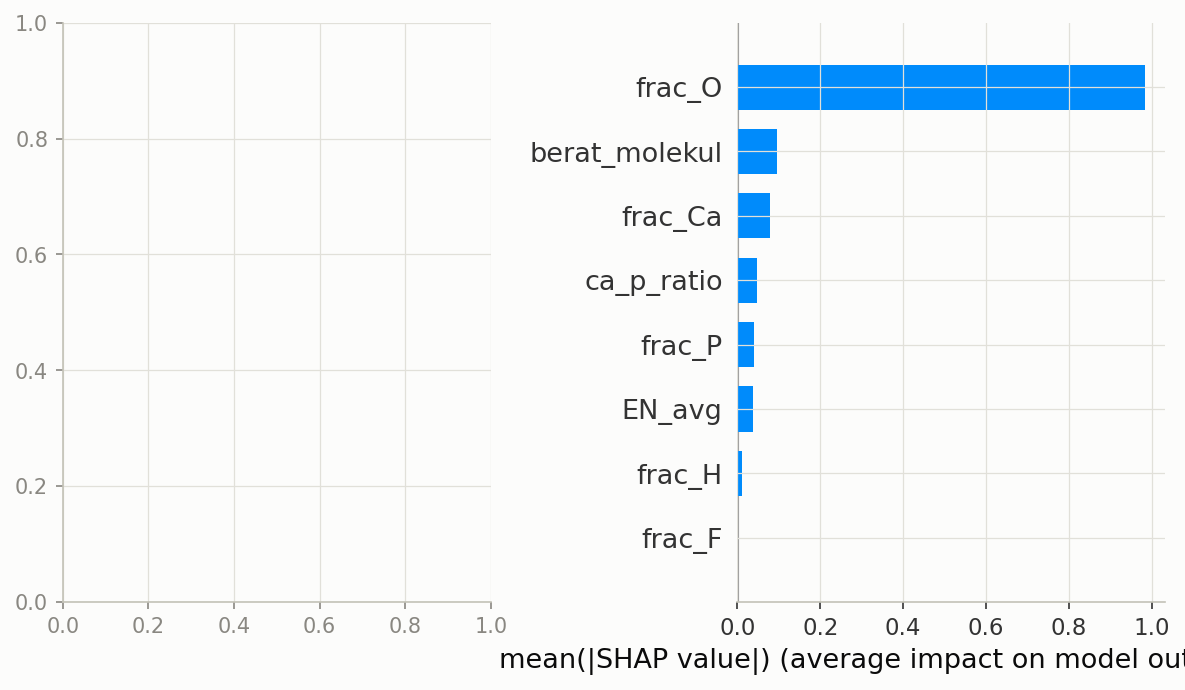
\includegraphics[width=0.60\textwidth]{fig_shap_bar_eform.png}
\caption{SHAP feature importance for the composition-only formation-energy model.}
\label{fig:shap}
\end{figure}

\subsection{Validation against independent experimental data}
\textbf{Dataset quality control.} Table~\ref{tab:val} compares \emph{database values} with experimental literature; it verifies the data sources rather than the models. The agreement is good (densities within 2.9\%; $\alpha$-TCP lattice parameters reproduced to $\leq 0.03\%$ because COD stores the very structures those literature values were derived from---a QC check, not an independent test). AFLOW reports TCP in the R-3m supergroup with density $+10.9$\% above experiment, a typical GGA overbinding artifact recorded as a source-specific limitation.

\textbf{Independent model validation.} The genuine test of the framework is whether the \emph{machine-learning predictions}---trained solely on database entries, using composition-only descriptors---reproduce experimental quantities for phases the models never saw. Table~\ref{tab:bench} benchmarks the nested SVR (formation energy) and the composition-only random forest (density) against standard experimental thermochemistry (Wagman/NBS formation enthalpies) and crystallographic densities for six calcium phosphate phases. The formation-energy model reproduces experiment with MAE 0.254 eV/atom (best: monetite $+0.08$, TTCP $+0.16$ eV/atom; largest: $\alpha$-TCP $+0.35$ eV/atom, reflecting the wide scatter of metastable-phase entries in the training sources). The composition-only density model reproduces experimental densities with MAE 0.177 g/cm$^3$---weaker than the formation-energy result, as expected for a packing-dominated property predicted from stoichiometry alone. In addition, at matching compositions the formation-energy model transfers across databases with $R^2 = 0.883$ (RMSE 0.385 eV/atom) on 280 OQMD entries.

\begin{table}[ht]
\centering\small
\caption{Independent validation of the machine-learning predictions against experimental data (standard formation enthalpies, Wagman/NBS; crystallographic densities). Composition-only descriptors; models trained exclusively on database entries.}
\label{tab:bench}
\begin{tabular}{lccccc}
\toprule
Phase & E$_f^{\mathrm{exp}}$ (eV/at) & E$_f^{\mathrm{pred}}$ & Density$^{\mathrm{exp}}$ & Density$^{\mathrm{pred}}$ & $\Delta$Density \\
\midrule
Hydroxyapatite & $-3.159$ & $-2.890$ & 3.16 & 3.056 & $-0.104$ \\
$\beta$-TCP & $-3.285$ & $-2.936$ & 3.07 & 3.365 & $+0.295$ \\
$\alpha$-TCP & $-3.289$ & $-2.936$ & 2.86 & 3.365 & $+0.505$ \\
TTCP & $-3.297$ & $-3.132$ & 3.05 & 3.060 & $+0.010$ \\
Monetite (DCPA) & $-2.686$ & $-2.608$ & 2.92 & 2.836 & $-0.084$ \\
Brushite (DCPD) & $-1.717$ & $-2.025$ & 2.31 & 2.247 & $-0.063$ \\
\midrule
MAE & & 0.254 & & & 0.177 \\
\bottomrule
\end{tabular}
\end{table}

\textbf{MLFF structural validation.} All five top candidates were relaxed with the universal machine-learning force field MACE-MP-0 (medium, float64): four of five are essentially at their energy minimum (cell-volume change $\leq 0.4\%$; TTCP $+3.0\%$), and the single-crystal stiffness falls in a narrow band ($E = 206$--$220$ GPa, $K = 127$--$139$ GPa, $\nu \approx 0.23$), consistent with dense apatitic ceramics (MLFF stiffness is known to be systematically high; definitive DFT runs await cluster resources). Applying Gibson--Ashby scaling, scaffolds fabricated from these candidates require roughly \textbf{70--78\% porosity} to match the 10--20 GPa modulus range of cortical bone---a concrete design specification for additive manufacturing.


\begin{table}[ht]
\centering\small
\caption{Dataset quality control: database values versus experimental literature. This table verifies the data sources; it does not validate the machine-learning models (see Table~\ref{tab:bench}).}
\label{tab:val}
\begin{tabular}{llccc}
\toprule
Phase & Property & This work & Literature & Deviation \\
\midrule
Hydroxyapatite & density (g/cm$^3$) & 3.178 & 3.16 & $+0.6$\% \\
 & E$_f$ (eV/atom) & $-3.223$ & $-3.15$ & $+2.3$\% \\
Fluorapatite & density (g/cm$^3$) & 3.104 & 3.19 & $-2.7$\% \\
 & E$_f$ (eV/atom) & $-3.42$ & $-3.39$ & $+0.9$\% \\
Carbonated apatite & density (g/cm$^3$) & 3.053 & 3.0 & $+1.8$\% \\
TTCP & density (g/cm$^3$) & 2.98--3.08 & 3.05 & $-2.4$\% to $+1.0$\% \\
$\beta$-TCP (R3c) & $a$ (\AA) & 10.449 & 10.44 & $+0.1$\% \\
 & $c$ (\AA) & 37.448 & 37.38 & $+0.2$\% \\
 & density (g/cm$^3$) & 3.04 & 3.07 & $-1.1$\% \\
$\alpha$-TCP (P21/a) & $a, b, c$ (\AA) & 12.887, 27.28, 15.219 & 12.89, 27.28, 15.22 & $\leq 0.03$\% \\
 & density (g/cm$^3$) & 2.86 & 2.86 & $+0.1$\% \\
\bottomrule
\end{tabular}
\end{table}

%=============================================================
\section{Discussion}

The ranking should be read for what it is. The criteria encode bone-tissue design requirements---stability, a density band covering all clinically processable calcium phosphate ceramics, proximity of Ca/P to bone mineral, and stiffness---so the top ranks are apatitic \emph{by construction}, not by surprise. We therefore make no claim of ``rediscovering'' the clinical hierarchy. What the ranking does deliver is a principled ordering within the design space, and it places clinically meaningful phases correctly: fluorapatite, carbonated apatite, $\beta$-TCP (rank 3), and hydroxyapatite lead, while tetracalcium phosphate (rank 6) and monetite (rank 12)---the two setting components of the classic calcium phosphate cements---and octacalcium phosphate (rank 15) sit inside the shortlist. $\beta$-TCP's presence in the top ranks rests on thermodynamic and compositional criteria; its distinctive clinical virtue, \emph{resorbability}, is still not represented by any criterion, and no resorption-sensitive ordering should be inferred from this ranking. Biphasic calcium phosphate (BCP) is a composite of hydroxyapatite and $\beta$-TCP rather than a single phase; both constituents are present in the candidate pool. Fluorapatite is standard in dental restoratives, and TTCP is the setting component of clinical calcium phosphate cements. The clearest framework limitation---and the most actionable direction for the next iteration---is therefore a resorption/solubility criterion derived from experiment or simulation, which would rank resorbable phases by their clinical merit rather than by stability alone.

Several limitations are worth noting, and we state them plainly because they bound what the framework can currently claim. \emph{Accuracy.} The honest composition-only models reach MAE 0.27 eV/atom (formation energy) and 0.26 g/cm$^3$ (density)---well behind graph-neural-network state of the art (CGCNN, MEGNet, M3GNet/CHGNet report MAE $\approx$ 0.03--0.1 eV/atom on benchmark sets). Our contribution is therefore the auditable, leakage-resistant \emph{pipeline} rather than regression accuracy; upgrading the surrogate to a GNN or a universal MLFF is a straightforward next step that we leave to future work. An earlier internal target ($R^2 \geq 0.85$) was set without a leakage analysis and is withdrawn as arbitrary. \emph{Leakage controls.} Reduced-formula grouping, nested CV, and composition-only features materially lowered reported scores (e.g., formation-energy $R^2$ from 0.87 to 0.48 in the discovery setting)---we report the conservative numbers throughout. \emph{Data.} Computed elastic moduli are scarce ($n=9$), so criterion C4 relies on median imputation; an MLFF (MACE-MP-0) pre-validation confirms candidate stability and yields porosity design targets (70--78\%), while definitive DFT validation awaits cluster resources (inputs prepared). The band gap is not predictable from composition descriptors ($R^2<0$). The dataset is source-biased (94\% same-source nearest neighbors); the ``external'' OQMD test is a same-composition cross-database transfer test rather than composition extrapolation, and the ranking uses absolute formation energies, which slightly penalizes AFLOW entries whose scale is offset by up to 0.8 eV/atom (a documented source artifact). The suitability label is a semi-deterministic function of its own features and was withdrawn as a predictive claim and as an MCDM criterion.

From an engineering standpoint, the framework is fully replicable: pinned dependencies (requirements.txt), a single orchestrator (run\_all), a versioned dataset with SHA-256 checksums, and open-source Python tooling. It is readily transferable to other material systems, supporting the AMREC roadmap toward an AI-assisted biomaterial discovery platform.

%=============================================================
\section{Conclusion}

We developed an end-to-end, replicable Materials Informatics framework that integrates five open databases, descriptor engineering with multicollinearity control, leakage-resistant machine learning (reduced-formula grouping, nested cross-validation, composition-only descriptors), multi-objective ranking (TOPSIS/VIKOR with entropy-based sensitivity analysis), and SHAP-based interpretability. The framework assembles a dataset of 2{,}885 entries (950 unique compositions) and delivers models whose predictions reproduce experimental thermochemistry: formation energies of six calcium phosphate phases with MAE 0.25 eV/atom, and densities with MAE 0.18 g/cm$^3$. These accuracies are modest compared with graph-neural-network state of the art, and we report them together with the leakage analysis that defines them. The multi-objective ranking, whose criteria are explicitly derived from bone-tissue design requirements, places fluorapatite, carbonated apatite, hydroxyapatite, and tetracalcium phosphate (together with its cement co-component monetite) at the top of a transparent candidate list---$\beta$-TCP enters the shortlist once its Ca/P and density are represented fairly---and the analysis exposes the framework's clearest gap: a missing resorption criterion. MLFF structural pre-validation confirms the stability of the top candidates and yields a porosity design target of 70--78\% for cortical-bone stiffness; definitive DFT validation inputs are prepared. The framework's value is methodological: a trustworthy, auditable screening pipeline with explicit, quantified limitations, ready to absorb stronger surrogates (GNNs, MLFFs) and further criteria.

%=============================================================
\section*{Acknowledgments}
This work is supported by the Universitas Airlangga Research Group Grant (PRGF Discovery Research, 2027) through the Advanced Materials and Renewable Energy Conversion (AMREC) research group. The authors thank the Materials Project, AFLOW, COD, PubChem, and OQMD communities for open data.

\section*{CRediT authorship contribution statement}
\textbf{Soegianto Soelistiono:} conceptualization, methodology, supervision, writing---original draft, writing---review \& editing. \textbf{Herri Trilaksana:} validation, formal analysis (physicochemical interpretation), writing---review \& editing. \textbf{Yhosep Gita Yhun Yhuwana:} software, data curation, formal analysis (machine learning), writing---review \& editing. \textbf{Bernardi Pranggono:} methodology (AI/ML advisory), writing---review \& editing.

\section*{Declaration of competing interest}
The authors declare that they have no known competing financial interests or personal relationships that could have appeared to influence the work reported in this paper.

\section*{Data and code availability}
The consolidated dataset, descriptor table, candidate ranking, per-stage reports, and all scripts are available in the project repository (git-tracked; dataset snapshot with SHA-256 checksums in data/versions/). The Materials Project subset is CC-BY 4.0; COD is CC0; AFLOW and OQMD data require citation of their respective references.

\begin{thebibliography}{26}
\bibitem{farag2023} Farag MM. Recent trends on biomaterials for tissue regeneration applications: review. \textit{J Mater Sci}. 2023;58:527--558.
\bibitem{premananth2024} Prem Ananth K, Jayram ND. A comprehensive review of 3D printing techniques for biomaterial-based scaffold fabrication in bone tissue engineering. \textit{Ann 3D Print Med}. 2024;13:100141.
\bibitem{vaiani2023} Vaiani L, Boccaccio A, Uva AE, et al. Ceramic materials for biomedical applications: an overview on properties and fabrication processes. \textit{J Funct Biomater}. 2023;14:146.
\bibitem{omigbodun2024} Omigbodun FT, Osa-Uwagboe N, Udu AG, Oladapo BI. Leveraging machine learning for optimized mechanical properties and 3D printing of PLA/cHAP for bone implant. \textit{Biomimetics}. 2024;9(10):587.
\bibitem{zhu2025} Zhu S, Sun H, Mu T, Richel A. Research progress in 3D printed biobased and biodegradable polyester/ceramic composite materials. \textit{ACS Appl Mater Interfaces}. 2025;17(2):2791--2813.
\bibitem{hou2026} Hou B, Yang X, Li Y, Wong RCW. Multiscale biomechanics-driven design pipelines for reconstructive bone scaffolds. \textit{npj Biol Phys Mech}. 2026;3(1).
\bibitem{vasudev2026} Vasudev H, Mehta A. Advanced manufacturing of biomedical scaffolds: modeling, simulation and process optimization approaches. \textit{Glob Clin Eng J}. 2026;8(2):35--56.
\bibitem{martelli2025} Martelli A, Bellucci D, Cannillo V. The role of artificial intelligence in biomaterials science: a review. \textit{Polymers (Basel)}. 2025;17(19):2668.
\bibitem{logeshwaran2024} Logeshwaran A, Elsen R, Nayak S. Artificial intelligence-based 3D printing strategies for bone scaffold fabrication and its application in preclinical and clinical investigations. \textit{ACS Biomater Sci Eng}. 2024;10(2):677--696.
\bibitem{gokcekuyu2024} Gokcekuyu Y, Ekinci F, Guzel MS, et al. Artificial intelligence in biomaterials: a comprehensive review. \textit{Appl Sci}. 2024;14:6590.
\bibitem{kang2023} Kang S, Kim M, Sun J, et al. Prediction of protein aggregation propensity via data-driven approaches. \textit{ACS Biomater Sci Eng}. 2023;9(11):6451--6463.
\bibitem{kalejaye2024} Kalejaye L, Wu IE, Terry T, et al. DeepSP: deep learning-based spatial properties to predict monoclonal antibody stability. \textit{Comput Struct Biotechnol J}. 2024;23:2220--2229.
\bibitem{hayashi2023} Hayashi Y, Nakano Y, Marumo Y, et al. A data-driven approach to predicting tablet properties after accelerated test using raw material property database and machine learning. \textit{Chem Pharm Bull (Tokyo)}. 2023;71(6):406--415.
\bibitem{nizamuddin2025} Nizamuddin SF, Ikramuddin M, Dhore NS. Artificial intelligence in pharmaceutical sciences: transforming drug discovery, formulation, and manufacturing. \textit{Mediterr J Med Res}. 2025;2(4):269--275.
\bibitem{han2025} Han Y, Kim DH, Pack SP. Nanomaterials in drug delivery: leveraging artificial intelligence and big data for predictive design. \textit{Int J Mol Sci}. 2025;26(22):11121.
\bibitem{vora2023} Vora LK, Gholap AD, Jetha K, et al. Artificial intelligence in pharmaceutical technology and drug delivery design. \textit{Pharmaceutics}. 2023;15(7):1916.
\bibitem{gholap2024} Gholap AD, Uddin MJ, Faiyazuddin M, et al. Advances in artificial intelligence for drug delivery and development: a comprehensive review. \textit{Comput Biol Med}. 2024;178:108702.
\bibitem{soelistiono2026} Soelistiono S. Data-driven discovery of calcium-phosphate biomaterial scaffolds using materials informatics and machine learning clustering. \textit{Int J Appl Pharm Life Sci}. 2026.
\bibitem{jain2013} Jain A, Ong SP, Hautier G, et al. Commentary: The Materials Project: a materials genome approach to accelerating materials innovation. \textit{APL Mater}. 2013;1:011002.
\bibitem{curtarolo2012} Curtarolo S, Setyawan W, Hart GLW, et al. AFLOW: an automatic framework for high-throughput materials discovery. \textit{Comput Mater Sci}. 2012;58:218--226.
\bibitem{kirklin2015} Kirklin S, Saal JE, Meredig B, et al. The Open Quantum Materials Database (OQMD): assessing the accuracy of DFT formation energies. \textit{npj Comput Mater}. 2015;1:15010.
\bibitem{grazulis2009} Gra\v{z}ulis S, Chateigner D, Downs RT, et al. Crystallography Open Database --- an open-access collection of crystal structures. \textit{J Appl Crystallogr}. 2009;42:726--729.
\bibitem{mathew1977} Mathew M, Schroeder LW, Dickens B, Brown WE. The crystal structure of $\alpha$-Ca$_3$(PO$_4$)$_2$. \textit{Acta Crystallogr B}. 1977;33:1325--1333.
\bibitem{dorozhkin} Dorozhkin SV. Calcium orthophosphates: applications in nature, biology, and medicine. \textit{Pan Stanford Publishing}; 2012.
\bibitem{lundberg2017} Lundberg SM, Lee S-I. A unified approach to interpreting model predictions. \textit{Adv Neural Inf Process Syst}. 2017;30.
\end{thebibliography}

\end{document}
